\subsection*{Algorithm Track Baseline Results}

% TODO if time: update section structure clarity with bolded presentation of main points

% Given our first itereation of the algorithmic track, we report baseline algorithm performance on each of the benchmarks using model architectures ranging from ANNs commonly used in deep-learning, to SNNs and reservoir networks. Each benchmark is evaluated with two significantly differing algorithm baselines, and we extract baseline comparisons, trends, and motivations towards future research. 

In our first iteration of the algorithmic track, we report baseline algorithm performance on each benchmark using various model architectures, including artificial neural networks commonly used in deep learning, spiking neural networks, and reservoir networks. We evaluate each benchmark with two substantially different algorithm baselines. From these evaluations, we extract baseline comparisons, identify trends, and uncover motivations for future research. Except for the event camera object detection task, each benchmark utilizes a novel data split, and all tasks use novel metric measurement. The presented baselines are a snapshot of the solution search space and will be starting points for leaderboards, thereby calling for further research to push the state of the art for each task. Detailed specifications of each of the baselines can be found in the Methods section.

    \subsubsection*{Keyword FSCIL}
    % \begin{table}[h]
% \centerline{
% \renewcommand{\arraystretch}{1.2}
% \begin{tabular}{|c|c|c|c|c|c|ccc|}
% \hline
% \multirow{2}{*}{Baseline} &
%   \multirow{2}{*}{\begin{tabular}[c]{@{}c@{}}Base\\ Accuracy\end{tabular}} &
%   \multirow{2}{*}{\begin{tabular}[c]{@{}c@{}}Footprint\\ (bytes)\end{tabular}} &
%   \multirow{2}{*}{\begin{tabular}[c]{@{}c@{}}Frequency\\ (Hz)\end{tabular}} &
%   \multirow{2}{*}{\begin{tabular}[c]{@{}c@{}}Connection\\ Sparsity\end{tabular}} &
%   \multirow{2}{*}{\begin{tabular}[c]{@{}c@{}}Activation\\ Sparsity\end{tabular}} &
%   \multicolumn{3}{c|}{SynOps (per sample)} \\ \cline{7-9} 
%         &       &          &    &     &       & \multicolumn{1}{c|}{Dense}    & \multicolumn{1}{c|}{Eff\_MACs} & Eff\_ACs \\ \hline
% M5 ANN & 97.36\% & $6.03 \times 10^6$ & 1 & 0.0 & 0.856 & \multicolumn{1}{c|}{$2.44 \times 10^9$} & \multicolumn{1}{c|}{$1.16 \times 10^8$}  & 0 \\ \hline
% SNN  & 93.77\% & $1.35 \times 10^7$ & 200 & 0.0 & 0.899 & \multicolumn{1}{c|}{$5.13 \times 10^9$} & \multicolumn{1}{c|}{0.0}  & $6.08 \times 10^8$ \\ \hline
% \end{tabular}
% }
% \caption{Baseline results for the keyword few-shot class-incremental learning task.}
%     \label{tab:FSCIL_resuls}
% \end{table}

% \begin{table}[ht]
% \centerline{
% \renewcommand{\arraystretch}{1.3}
% \begin{tabular}{c|cccccccc} \thickhline
% \multirow{2}{*}{Baseline} &
%   \multirow{2}{*}{\begin{tabular}[c]{@{}c@{}}Pre-training\\ Accuracy\end{tabular}} &
%   \multirow{2}{*}{\begin{tabular}[c]{@{}c@{}}Footprint\\ (bytes)\end{tabular}} &
%   \multirow{2}{*}{\begin{tabular}[c]{@{}c@{}}Frequency\\ (Hz)\end{tabular}} &
%   \multirow{2}{*}{\begin{tabular}[c]{@{}c@{}}Connection\\ Sparsity\end{tabular}} &
%   \multirow{2}{*}{\begin{tabular}[c]{@{}c@{}}Activation\\ Sparsity\end{tabular}} &
%   \multicolumn{3}{c}{SynOps (per sample)} \\ \cline{7-9} 
%         &       &          &    &     &       & \multicolumn{1}{c}{Dense}    & \multicolumn{1}{c}{Eff\_MACs} & Eff\_ACs \\ \hline
% M5 ANN & 97.36\% & $6.03 \times 10^6$ & 1 & 0.0 & 0.856 & \multicolumn{1}{c}{$2.44 \times 10^9$} & \multicolumn{1}{c}{$1.16 \times 10^8$}  & 0 \\ 
% SNN  & 93.77\% & $1.35 \times 10^7$ & 200 & 0.0 & 0.899 & \multicolumn{1}{c}{$5.13 \times 10^9$} & \multicolumn{1}{c}{0}  & $6.08 \times 10^8$ \\ \thickhline
% \end{tabular}
% }
% \caption{Baseline results for the keyword few-shot class-incremental learning task. Here, accuracy on the base 100 classes is reported. Accuracy across incremental sessions is shown in Figure~\ref{fig:mswc_acc_per_session}. \TODO{Update the synops with the correct synops} \JY{? Change to Compute Frequency, SynOps per compute}}
%     \label{tab:FSCIL_resuls}
% \end{table}



\begin{table}[ht]
\centerline{
\renewcommand{\arraystretch}{1.3}
\begin{tabular}{c|cccccccc} \thickhline
\multirow{2}{*}{Baseline} &

  \multirow{2}{*}{\begin{tabular}[c]{@{}c@{}}Accuracy\\ (Base / Session Avg)\end{tabular}} &
  \multirow{2}{*}{\begin{tabular}[c]{@{}c@{}}Footprint\\ (bytes)\end{tabular}} &
  \multirow{2}{*}{\begin{tabular}[c]{@{}c@{}}Model Exec.\\ Rate (Hz)\end{tabular}} &
  \multirow{2}{*}{\begin{tabular}[c]{@{}c@{}}Connection\\ Sparsity\end{tabular}} &
  \multirow{2}{*}{\begin{tabular}[c]{@{}c@{}}Activation\\ Sparsity\end{tabular}} &
  \multicolumn{3}{c}{SynOps (per model exec.)} \\ \cline{7-9} 
        &       &          &    &     &       & \multicolumn{1}{c}{Dense}    & \multicolumn{1}{c}{Eff\_MACs} & Eff\_ACs \\ \hline
M5 ANN & (97.09\% / 89.27\%) & $6.03 \times 10^6$ & 1 & 0.0 & 0.783 & \multicolumn{1}{c}{$2.59 \times 10^7$} & \multicolumn{1}{c}{$7.85 \times 10^6$}  & 0 \\ 
SNN  & (93.48\% / 75.27\%) & $1.36 \times 10^7$ & 200 & 0.0 & 0.916 & \multicolumn{1}{c}{$3.39 \times 10^6$} & \multicolumn{1}{c}{0}  & $3.65 \times 10^5$ \\ \thickhline
\end{tabular}
}
\caption{Baseline results for the keyword few-shot class-incremental learning task. Base accuracy refers to accuracy on the 100 base classes after pre-training while session average accuracy is the average accuracy over all sessions for the corresponding prototypical baseline. The detailed accuracy per session for the different baselines are shown in Figure~\ref{fig:mswc_acc_per_session}.}
    \label{tab:FSCIL_results}
\end{table}



% WEIGHT CONSOLIDATION RESULTS

% \begin{table}[ht]
% \centerline{
% \renewcommand{\arraystretch}{1.3}
% \begin{tabular}{c|cccccccc} \thickhline
% \multirow{2}{*}{Baseline} &
%   \multirow{2}{*}{\begin{tabular}[c]{@{}c@{}}Pre-training\\ Accuracy\end{tabular}} &
%   \multirow{2}{*}{\begin{tabular}[c]{@{}c@{}}Footprint\\ (bytes)\end{tabular}} &
%   \multirow{2}{*}{\begin{tabular}[c]{@{}c@{}}Model Exec.\\ Rate (Hz)\end{tabular}} &
%   \multirow{2}{*}{\begin{tabular}[c]{@{}c@{}}Connection\\ Sparsity\end{tabular}} &
%   \multirow{2}{*}{\begin{tabular}[c]{@{}c@{}}Activation\\ Sparsity\end{tabular}} &
%   \multicolumn{3}{c}{SynOps (per model exec.)} \\ \cline{7-9} 
%         &       &          &    &     &       & \multicolumn{1}{c}{Dense}    & \multicolumn{1}{c}{Eff\_MACs} & Eff\_ACs \\ \hline
% M5 ANN & 97.36\% & $6.03 \times 10^6$ & 1 & 0.0 & 0.856 & \multicolumn{1}{c}{$2.59 \times 10^7$} & \multicolumn{1}{c}{$5.75 \times 10^6$}  & 0 \\ 
% SNN  & 93.77\% & $1.35 \times 10^7$ & 200 & 0.0 & 0.916 & \multicolumn{1}{c}{$3.39 \times 10^6$} & \multicolumn{1}{c}{0}  & $3.65 \times 10^5$ \\ \thickhline
% \end{tabular}
% }
% \caption{Baseline results for the keyword few-shot class-incremental learning task. Here, accuracy after pre-training on the base 100 classes is reported. Accuracy across incremental sessions is shown in Figure~\ref{fig:mswc_acc_per_session}.}
%     \label{tab:FSCIL_results}
% \end{table}

    The keyword FSCIL task has an ANN and SNN baseline, using different model architectures:
    
    \begin{itemize}
        \item \textbf{M5 ANN} -- The ANN baseline uses a tuned version of the M5 deep convolutional network architecture~\cite{dai2016deep}, with samples pre-processed into Mel-frequency cepstral coefficients (MFCC). The network contains four successive convolution-normalization-pooling layers, followed by a readout fully-connected layer. Each model execution (forward pass) uses the data from the full pre-processed sample, and convolution kernels are applied over the temporal dimension of the samples. This is reported as a 1~Hz model execution rate.
        % Convolutional kernels are applied over the temporal dimension of the samples. 

        \item \textbf{SNN} -- The SNN baseline uses a recurrent SNN with adaptive leaky integrate-and-fire (LIF) neurons and heterogeneous time constants~\cite{bittar22surrogate}. The SNN consists of two recurrent adaptive LIF layers and one linear output layer.
        Audio samples are pre-processed to binary spike trains using Speech2Spikes~\cite{stewart23speech2spikes}, which relies on a Mel Spectrogram with the same parameters as the MFCC of the ANN baseline. Each input timestep to the model represents 5~ms of audio data, thus the model has a 200~Hz model execution rate. Output neuron activations are summed over time to produce the word class prediction.
    \end{itemize}

    % \begin{figure}[h]
    %             \centering
    %             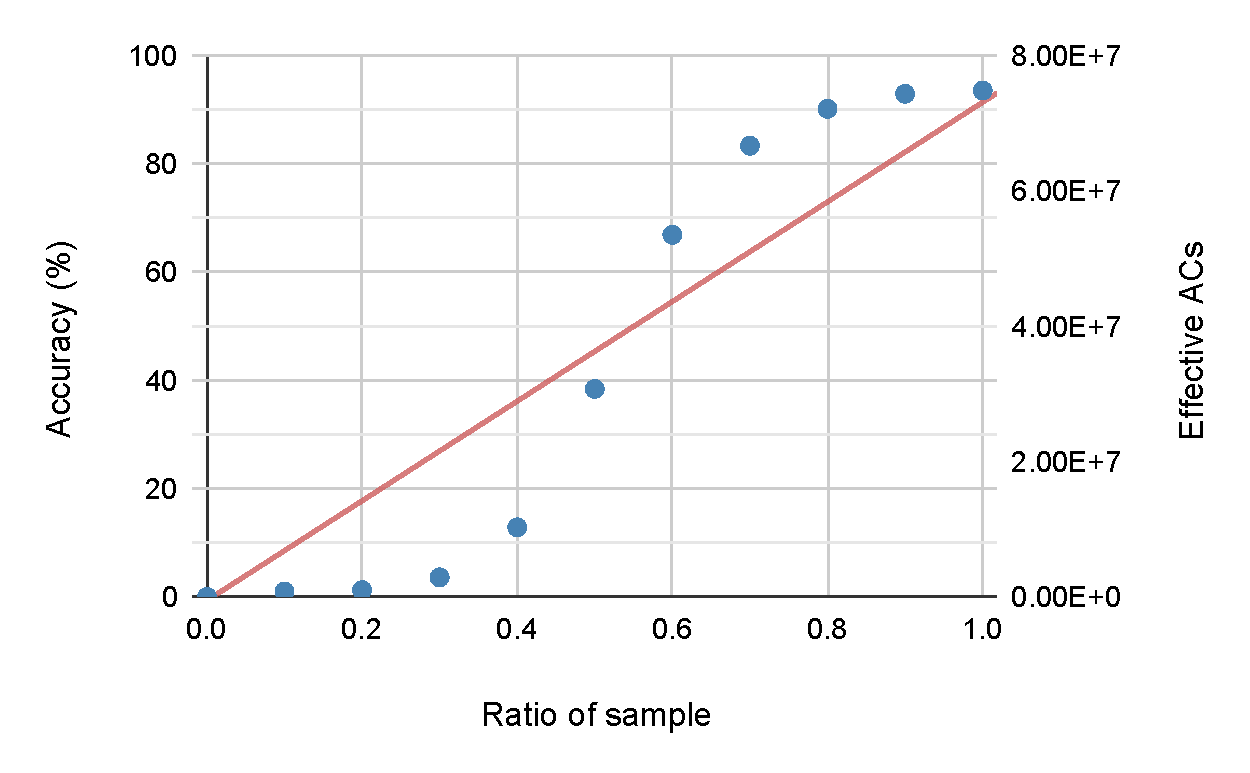
\includegraphics[width=.70\textwidth]{figures/snn_acc_compute_time.pdf}
    %             \caption{Test accuracy (blue) and aggregated effective ACs (red) of SNN on base classes using only the first portions of the keyword sample.}
    %         \label{fig:snn_acc_time}
    %     \end{figure}

% a base session with fixed classes, each with abundant training data, is used to train an initial model. Then, successive incremental training sessions introduce new classes in a few-shot learning scenario. In each session, only the current session classes are available to the model for training. After each incremental training session, the model is evaluated on all previously seen classes, including the base classes. Therefore, the model has to learn new classes while retaining knowledge about the previously learned ones. 

    % The keyword FSCIL task first uses a base dataset consisting of 100 base classes with abundant training data to pre-train models before proceeding with incremental learning on 100 extra classes. 
    After pre-training using standard batched training, the ANN and SNN baseline networks reach high accuracies on the base classes of 97.09\% and 93.48\%, respectively.
    % \red{The SNN solution, including the pre-processing, processes one input timestep at a time with a frequency of 200~Hz, compared to the ANN which requires a full one second sample to pass through the model. While the number of effective operations per-sample is lower for the ANN baseline, the SNN distributes computation temporally over 200 timesteps, thus its effective operations per model execution is one order of magnitude lower ($3.65 \times 10^5$).}
    As reported by the model execution rate metric, the SNN baseline computes each sample over 200 passes, using an order of magnitude fewer effective AC synaptic operations compared to the ANN baseline's effective MACs per model execution.
    Considering both the model execution rate and synaptic operation metrics, the number of aggregated ACs over the length of the sample ($200 * 3.65 \times 10^5 = 7.30 \times 10^7$) exceeds the Dense and effective MAC operations necessary for the ANN baseline, which spatially flattens the sample and processes it in one model execution.
    However, outside of the static-length keyword classification scenario, the low-cost per-execution temporal processing of SNNs can enable efficient, always-on, high-frequency prediction capabilities in deployed continuous audio recognition scenarios. 

    % Furthermore, the temporal processing of the SNN has capabilities to produce predictions before the sample is completed. 
    % Figure~\ref{fig:snn_acc_time} demonstrates that the SNN reaches 90\% accuracy using the first 80\% of the sample. Moreover, the number of aggregated effective ACs grows as a linear function of the sample ratio, demonstrating a compute reduction corresponding to the early prediction. Further research in online neuromorphic methods for fast time-to-prediction and compute-accuracy trade-offs\cite{jeffares2022spikeinspired} is enabled by the benchmark data features (see Methods section).
    

    \begin{figure}[ht]
                \centering
                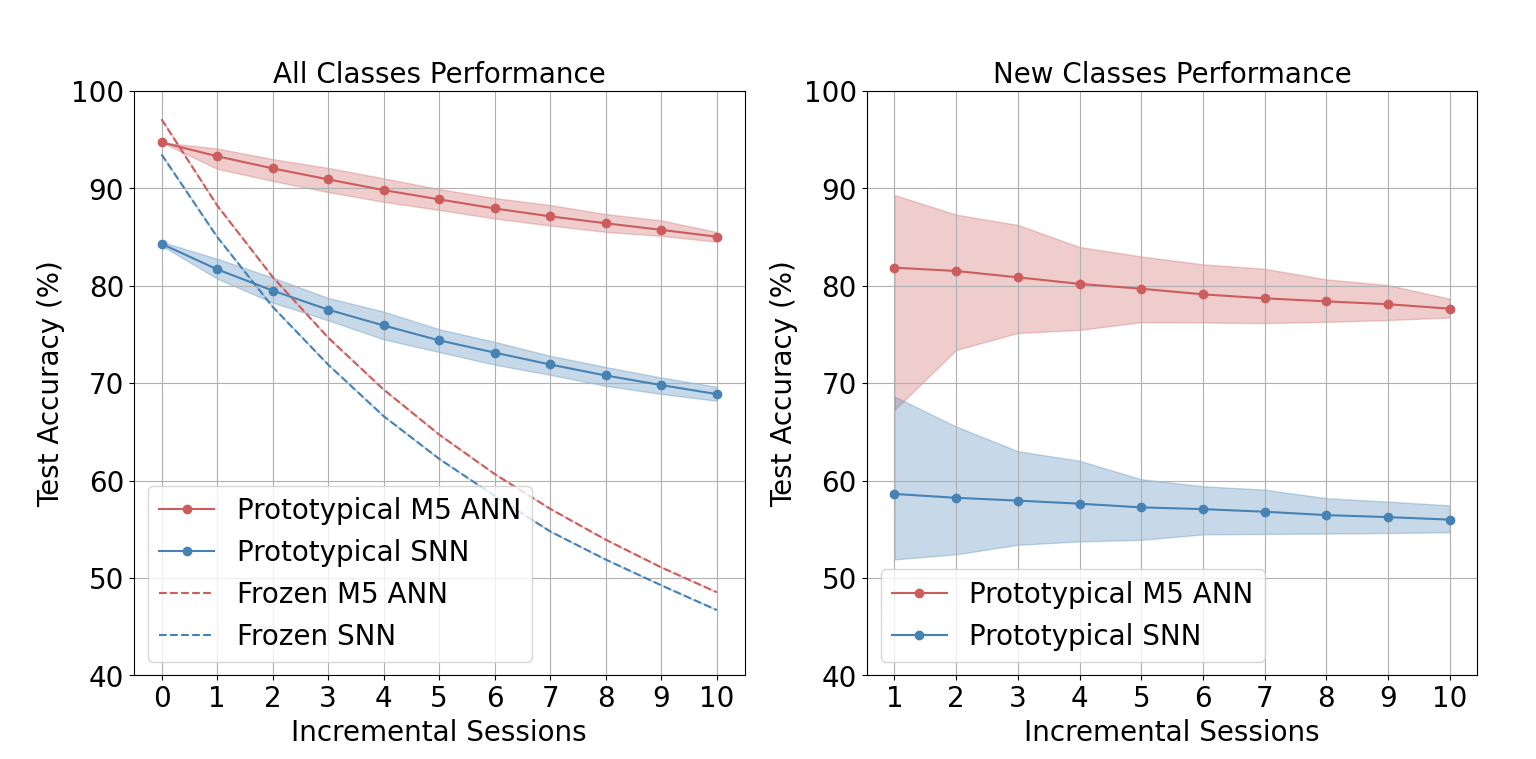
\includegraphics[width=\textwidth]{figures/FSCIL_proto.png}
                \caption{Test accuracy per session on the keyword FSCIL task for prototypical and frozen baselines, with the accuracy on both base classes and incrementally-learned classes (left), and accuracy on all incrementally-learned classes only (right). Incremental session 0 refers to the accuracy on base classes after pre-training only. Shaded area represents 5$^{th}$ and 95$^{th}$ percentile on 100 runs. Frozen baselines with no adaptation do not learn incremental classes and thus have a fixed 0\% accuracy for New Classes Performance. }
            \label{fig:mswc_acc_per_session}
        \end{figure}


    % For the incremental learning portion of the task, 10 successive sessions, each representing a new language, are presented to the model. Each session contains 10 new classes with 5 samples each (10-way 5-shot learning). This set-up 

% NEW VERSION WITH PROTOTYPES METHOD:

    % The 10-way, 5-shot class-incremental learning per incremental session poses the challenge of learning new classes while avoiding catastrophic forgetting, especially with the limited number of samples for new classes. We therefore present two reference solutions for both the ANN and SNN baselines: a \textbf{frozen} baseline with no weight updates in the incremental learning phase and a \textbf{prototypical} baseline that employs class prototypes~\cite{snell2017prototypical} for incremental learning. 
    % The frozen ANN and SNN have 0\% accuracy on incremental classes, and serve as reference for models which have no learning, but also no catastrophic forgetting of prior classes. 

    % In prototypical networks~\cite{snell2017prototypical}, all classes are associated with a \textit{prototype}, which is the average feature embedding, produced by the network before the readout classifier layer, over all training samples for each class. During inference, input samples are classified as the class corresponding to the prototype with the lowest squared Euclidean distance to the sample's embedding. Since computing this distance is equivalent to an affine operation on the feature embeddings~\cite{snell2017prototypical}, the prototypical network classifier can be expressed as a standard linear readout layer defined with respect to the prototype of each class. Thus, the final model consists of a prototype classifier output layer following the feature extracting hidden layers.

    % Although the original work on prototypical networks suggests a specific approach to train the feature extractor network~\cite{snell2017prototypical}, we employ standard pre-training with end-to-end backpropagation to enable high base class accuracy. After pre-training, the readout classifier layer is dropped, and the base classes prototypes and prototype layer are computed a-posteriori based on features from the hidden layers of the pre-trained network. This allows for common readout classification for base and incremental classes, however, it comes with an accuracy loss for base classes as the feature extraction in hidden layers is not trained with the classifier. 

    % The prototypical network approach is simple and computationally efficient, as no hyperparameters are used and parameters are not optimized, but instead calculated directly. 
    % Also, the prototypical evaluation method does not affect model complexity, as the prototypical classifier directly substitutes the default readout layer. Thus, the complexity results in Table~\ref{tab:FSCIL_results} empirically apply to both the frozen and prototypical models.

    % JY: compressed details from prior 4 paragraphs into this single paragraph, also compressed the following paragraphs
    We present two approaches for the incremental stage for both the ANN and SNN baselines. The \textit{frozen} models are locked after pre-training on base classes and have 0\% accuracy on all new incremental classes, providing a reference for models with no learning or catastrophic forgetting of prior classes. The \textit{prototypical} models employ a prototypical network~\cite{snell2017prototypical} for incremental learning, which is a feature-based clustering approach that can be implemented with a simple linear readout layer on top of the pre-trained network backbone. Prototypical weights and biases of prior and incremental classes are directly defined based on the average features of the corresponding class and directly substitute pre-trained readout layer parameters.  The complexity results in Table~\ref{tab:FSCIL_results} thus empirically apply to both the frozen and prototypical models.
    
    The test accuracy for the baseline models over all sessions, as well as the test accuracy on only the new incrementally-learned classes, are shown in Figure~\ref{fig:mswc_acc_per_session}.
    Using prototypical networks, the ANN model reaches 89.27\% accuracy on average over all sessions, demonstrating significant greater performance of 21.41 accuracy points with respect to the frozen model. The accuracy on new classes, averaged over all incremental sessions, is 79.61\%.
    The SNN prototypical baseline, on the other hand, reaches 75.27\% accuracy on average over all sessions, surpassing the frozen SNN performance by 9.97 accuracy points, with an average accuracy on new classes over all sessions of 57.23\%. 

    The accuracy loss over the incremental sessions is similar between the ANN and SNN prototypical baselines. However, the lower overall accuracy of the SNN is largely due to the conversion from the original backpropagation-trained readout classifier, which is used in the frozen baseline, to the prototype readout classifier. 
    On the base classes (session 0 in Figure~\ref{fig:mswc_acc_per_session}), the ANN sees a drop of 2.37\% between the frozen and prototypical baselines, while the SNN has a larger drop of 9.17\%. 
    The larger drop indicates that our particular SNN baseline has a less general feature extraction than the ANN. This may be due to the challenges of backpropagation through time for online temporal inference to learn to extract long-term temporal keyword features with the chosen spiking recurrent model. Additionally, the Speech2Spikes~\cite{stewart23speech2spikes} pre-processing algorithm converting audio to spikes may also cause information loss. Overall, the keyword FSCIL benchmark presents opportunities for further research in learning methods, preprocessing, and model architectures for continual learning of temporal data. 

    % A significant part of the gap in performance between the SNN and ANN prototypical baselines is due to the conversion from backpropagation-trained readout layer to prototype layer after pre-training, as the further accuracy drop over sessions is quite similar. Although the ANN also sees a drop of 2.37\% between the frozen and prototypical baselines at session 0, the impact on the SNN is notably bigger with a drop of 9.17\% due to the conversion. This can be explained by a less general feature extraction obtained with the SNN. The first hypothesis for that is that the online nature of the SNN, along with backpropagation through time, despite its computational advantage is making it harder for the network to extract long-term temporal features for the selected keywords. Additionally the pre-processing algorithm used to convert Spectrograms to spikes can create a loss of information as it has not been fine-tuned for this task. We want present this remaining gap between keyword spotting SNN and CNN models as an incentive for the community to keep researching this challenge in the direction of more refined pre-processings for SNNs and better architectures to extract robust temporal features.


    % Altogether, we nonetheless showed the ability of both ANN and SNN networks to demonstrate some class-incremental learning capacities with the prototypical networks method on this new keyword classification FSCIL task. This should serve as a simple reference to explore a challenge that is pushing the required learning and embedding capacities of neural networks to their fullest in a temporal domain setup.


% WEIGHT CONSOLIDATION (OLD METHOD) VERSION BELOW

    
    % The 10-way, 5-shot class-incremental learning per incremental session poses the challenge of learning new classes while avoiding catastrophic forgetting, especially with the limited number of samples for new classes. We therefore present two reference solutions for both the ANN and SNN baselines: a \textbf{frozen} baseline with no weight updates in the incremental learning phase and a \textbf{consolidated} baseline that employs a weight consolidation method~\cite{pellegrini20latent} for incremental learning. 
    % The frozen ANN and SNN have 0\% accuracy on incremental classes, and serve as reference for models which have no learning, but also no catastrophic forgetting of prior classes. The weight consolidation method for the consolidated baselines incrementally learn new classes by training only weights corresponding to newly learned classes in the output layer, centering weights around zero based on the average of newly trained weights. 
    % Notably, the weight consolidation method does not affect model complexity, thus the results in Table~\ref{tab:FSCIL_results} empirically apply to the frozen and consolidated models.
    
    % The \textbf{frozen} baselines keep the same parameters obtained in pre-training throughout all the incremental sessions. During pre-training, the 200 output neurons for the whole 200 final classes are present. Thus the \textbf{frozen} baselines present a 0 accuracy on all new classes as output weights to . They are nonetheless a relevant reference as 
    
    % the ANN baseline is trained with weight consolidation~\cite{pellegrini20latent} to learn the new classes. During each session of the FSCIL task, only the weights corresponding to the newly learned classes in the output layer of the model are trained using the few-shot training samples. Moreover, after all training sessions, including the pre-training, these weights are centered around zero based on the average on the newly trained weights. The test accuracy over sessions, as well as accuracy on only the incrementally-learned classes, is shown in Figure~\ref{fig:mswc_acc_per_session}.

    
    % The test accuracy for the baselines over all sessions, as well as the test accuracy on only the incrementally-learned classes, can be found in Figure~\ref{fig:mswc_acc_per_session}. 
    % Using weight consolidation, the ANN model reaches 85.70\% accuracy on average over all sessions, demonstrating significant relative improvement of 25.70\% with respect to the frozen model. This demonstrates the ability of the ANN solution to learn new classes from few-shot examples while limiting forgetting of previous classes. The accuracy on incremental classes, on average, is 64.48\%.

    % \red{For the SNN model, the same weight consolidation method used for the ANN did not provide an improvement on the default baseline with no incremental training, as the network either could not manage to learn new classes at all or new class predictions overshadowed the prediction of old classes and caused catastrophic forgetting. We therefore only provide the non-learning FSCIL baseline for the SNN model at this point, and motivate future research in adaptive few-shot, incremental learning in SNNs.}

    % The SNN baseline, on the other hand, reaches 66.23\% accuracy on average over all sessions, improving the frozen SNN performance by 1.43\% with an average accuracy on incremental classes of 3.87\%. \note{See note in Figure 4, exploring a better SNN baseline.} The observed limitation of weight consolidation with the SNN is a high sensitivity to the learning rate employed in incremental sessions. Low learning rates hinder the ability to learn new classes while greater rates cause catastrophic forgetting as the newly learned classes overshadow prior ones. 
    % The SNN baseline motivates further research into model architectures and learning rules for developing solutions to the FSCIL problem.
    % Contrary to the ANN solution, a sweep spot of learning rate with this weight consolidation could not be found. We make the hypothesis that this is due to the more sensitive nature of spiking neurons and of backpropagation through time, and incite the community to face this challenge to provide a more efficient solution to the FSCIL problem.

    

    % JY: we don't really have an SNN training method, so no need to mention training complexity?
    % We further note that the NeuroBench benchmarks do not yet specify metrics for model training complexity - all complexity metrics refer to model inference only. Future NeuroBench iterations will look towards training metrics, including potential solution-specific metrics for online weight adaptation, which can be measured during the few-shot training of the FSCIL task.

    
    \subsubsection*{Event Camera Object Detection}

    % \begin{table}[h]
% \centerline{
% \renewcommand{\arraystretch}{1.2}
% \begin{tabular}{|c|c|c|c|c|c|ccc|}
% \hline
% \multirow{2}{*}{Baseline} &
%   \multirow{2}{*}{COCO mAP} &
%   \multirow{2}{*}{\begin{tabular}[c]{@{}c@{}}Footprint\\ (bytes)\end{tabular}} &
%   \multirow{2}{*}{\begin{tabular}[c]{@{}c@{}}Frequency\\ (Hz)\end{tabular}} &
%   \multirow{2}{*}{\begin{tabular}[c]{@{}c@{}}Connection\\ Sparsity\end{tabular}} &
%   \multirow{2}{*}{\begin{tabular}[c]{@{}c@{}}Activation\\ Sparsity\end{tabular}} &
%   \multicolumn{3}{c|}{SynOps} \\ \cline{7-9} 
%         &       &          &    &     &       & \multicolumn{1}{c|}{Dense}    & \multicolumn{1}{c|}{Eff\_MACs} & Eff\_ACs \\ \hline
% RED ANN & 0.429 & $9.13 \times 10^7$ & 20 & 0.0 & 0.634 & \multicolumn{1}{c|}{$2.84 \times 10^{11}$} & \multicolumn{1}{c|}{$2.48 \times 10^{11}$}  & 0 \\ \hline
% Hybrid  & 0.271 & $1.21 \times 10^7$ & 20 & 0.0 & 0.613 & \multicolumn{1}{c|}{$9.85 \times 10^{10}$} & \multicolumn{1}{c|}{$3.76\times 10^{10}$}  & $5.60\times10^8$ \\ \hline
% \end{tabular}
% }
% \caption{Baseline results for the event camera object detection task.}
%     \label{tab:ObjDet_resuls}
% \end{table}

\begin{table}[ht]
\centerline{
\renewcommand{\arraystretch}{1.3}
\begin{tabular}{c|cccccccc} \thickhline
\multirow{2}{*}{Baseline} &
  \multirow{2}{*}{\begin{tabular}[c]{@{}c@{}}mAP\end{tabular}} &
  \multirow{2}{*}{\begin{tabular}[c]{@{}c@{}}Footprint\\ (bytes)\end{tabular}} &
  \multirow{2}{*}{\begin{tabular}[c]{@{}c@{}}Model Exec.\\ Rate (Hz)\end{tabular}} &
  \multirow{2}{*}{\begin{tabular}[c]{@{}c@{}}Connection\\ Sparsity\end{tabular}} &
  \multirow{2}{*}{\begin{tabular}[c]{@{}c@{}}Activation\\ Sparsity\end{tabular}} &
  \multicolumn{3}{c}{SynOps (per model exec.)} \\ \cline{7-9} 
        &       &          &    &     &       & \multicolumn{1}{c}{Dense}    & \multicolumn{1}{c}{Eff\_MACs} & Eff\_ACs \\ \hline
RED ANN & 0.429 & $9.13 \times 10^7$ & 20 & 0.0 & 0.634 & \multicolumn{1}{c}{$2.84 \times 10^{11}$} & \multicolumn{1}{c}{$2.48 \times 10^{11}$}  & 0 \\
Hybrid  & 0.271 & $1.21 \times 10^7$ & 20 & 0.0 & 0.613 & \multicolumn{1}{c}{$9.85 \times 10^{10}$} & \multicolumn{1}{c}{$3.76\times 10^{10}$}  & $5.60\times10^8$ \\ \thickhline
\end{tabular}
}
\caption{Baseline results for the event camera object detection task.}
    \label{tab:ObjDet_resuls}
\end{table}

    The event camera object detection task reports a prior baseline, the RED ANN, and a novel conversion of the architecture to a hybrid ANN-SNN model:
    
    \begin{itemize}
        \item \textbf{RED ANN} -- The RED architecture \cite{Perot2020} consists of blocks of feed-forward squeeze-and-excite~\cite{hu18squeeze} convolutional layers followed by blocks of recurrent convolution-LSTM (ConvLSTM~\cite{shi15convlstm}) layers.
        % The feed-forward convolutional layer is the squeeze-and-excitation layer for better performance. The recurrent convolutional layer is the ConvLSTM layer for effective temporal learning. 
        A single-shot detection (SSD~\cite{Liu_2016}) head is used to predict the location and class of the bounding box based on multi-scale outputs from the recurrent layers. 
        %The RED architecture has activation sparsity in the feed-forward convolutional layers. However, due to the activation function used, the ConvLSTM layers output dense activations. 
        Raw event data is binned into 50 ms and pre-processed into time surfaces. 
        %The model is trained using the SSD loss function consisting of a regression term for box coordinates and a classification term for the class. The selection of the SSD loss terms is the same as in the RED paper.
        \item \textbf{Hybrid} -- The hybrid ANN-SNN architecture adopts feedforward LIF spiking neural layers to replace the ConvLSTM layers in RED, and shares the same feed-forward convolutional blocks as the RED. It uses the same input encoding method and SSD head as the RED model. 
        % The model shares the same input encoding method, object detection head, and training loss functions as the RED model.
    \end{itemize}

    Results for the two networks can be found in Table \ref{tab:ObjDet_resuls}. The RED ANN represents the current state-of-the-art correctness on the benchmark, at 0.429 mAP. The Hybrid network is a smaller network, reflected by the footprint and synaptic operations metrics measuring an order of magnitude smaller than for the RED ANN. The smaller size comes at the expense of lower correctness of 0.271 mAP.

    For the RED ANN, the activation sparsity metric (0.634) represents zero activations by the ReLU function for each neuron. From this, one may expect that the number of effective operations (operations with a nonzero activation and nonzero weight) would be around 35\% of dense operations, however the actual ratio is 87\%. This is due to the presence of normalization layers applied to activations before synaptic weight multiplication. Furthermore, neurons with lower activation frequency in the network tend to have a smaller fanout than neurons with high activation frequency. Thus, while activation sparsity alone can provide a proxy for the cost of the network, architectural characteristics may impede actual computation reduction, and the synaptic operations must be considered in tandem.

    The Hybrid network demonstrates a significant reduction in total effective operations against dense operations, outlining significant gains if deployed on specialized sparsity-aware hardware. However, for the particular network, the number of effective ACs, generated by the spiking neuron components, is two orders of magnitude smaller than the number of effective MACs within the ANN components. Such a hybrid network may not warrant specialized accumulation units, and the baseline motivates further research in hybrid networks with a larger proportion of spiking neuron activity compared to artificial neuron activity.

    % Lastly, the connection sparsity metrics for both models is zero, indicating opportunities in weight pruning and sparse recurrent layers.

    \subsubsection*{NHP Motor Prediction}
\input{tables/primate_reaching_baselines}

    Small fully-connected, feedforward networks were developed for the NHP motor prediction baselines:
    
    \begin{itemize}
        \item \textbf{ANN} -- In the ANN baseline, the cortical activity from the 50 most recent data samples is buffered to be used as network input. The network has two hidden layers and $2$ final outputs predicting $X$ and $Y$ velocities, with a fully-connected topology of $N_{ch}$-32-48-2, where $N_{ch}$ refers to the channels of cortical data (96 for NHP Indy, and 192 for NHP Loco). Batch normalization is applied after each hidden layer.
        
        \item \textbf{SNN} -- The SNN uses the data samples directly as input to the network, without buffering. It has a hidden layer of 50 LIF neurons, for a fully connected topology of $N_{ch}$-50-2 LIF neurons. The output neurons do not have a reset mechanism, and the membrane potential is directly read to produce the output velocities. 
        
        % \TODO{Layernorm SNN with three layers vs Paul SNN with only two layers} The SNNs, similar to ANNs used a temporal window of $T_{BW}=200$ ms for the prediction. Similar to ANN$\_$V2, it splits this window into $n_p=7$ subsets, each of which corresponded to a timestep of the SNN. \red{The firing rates in each subset were binarized and fed as input to the SNN} to eliminate multiplications. Unlike the ANN$\_$V2, the input dimension remained equal to $N_{ch}$, reducing memory. However, computations were increased since all the layers had to be run for $n_p$ timesteps. For each new prediction, the SNN was reinitialized to operate over $n_p$ timesteps even though the current temporal window had overlap with the previous one. The SNN employed a fully connected topology $N_{ch}$-32-48-2. Since the task was regression, the neuron in the last layer did not have a reset mechanism, and the membrane voltage at the last time was considered as the output. Each membrane voltage was scaled by a learnt parameter to match the range of $X$ and $Y$ velocities.
    \end{itemize}

Table \ref{tab:primate_results} shows the results for the ANN and SNN baselines, averaged between sessions from each NHP (Indy and Loco). The ANN and SNN are similar in footprint size and number of dense operations per model forward pass, and also reach comparable prediction quality based on $R^2$ score. Each model is small in footprint and operation count, demonstrating that this task can be solved by shallow edge networks, validating prior studies~\cite{willsey22realtime}.

Between the baselines, the SNN realizes similar correctness at significantly reduced complexity compared to the ANN. Extremely high activation sparsity in the SNN (0.998) directly translates to low effective accumulate operations, demonstrating the adequacy of stateful, binary-activation neuron models for sparse regression tasks. Meanwhile, similarly to the RED ANN in the event camera object detection task, activation sparsity in the ANN baseline does not translate to effective operation efficiency, as batch normalization is applied to activations before multiplication with synaptic weights.

\begin{figure} [ht]
\centering
\begin{subfigure}{.5\textwidth}
  \centering
  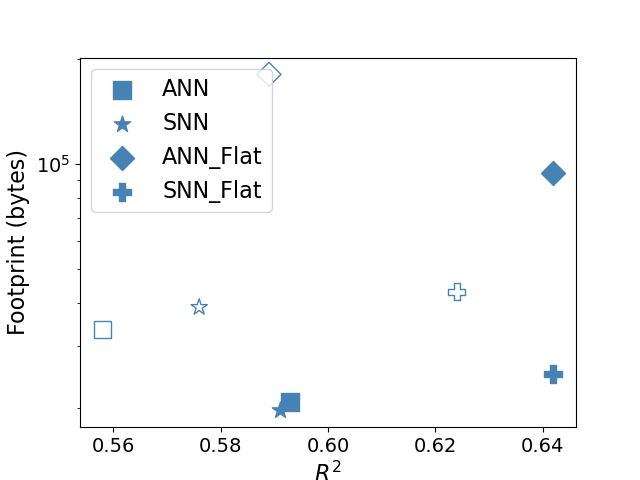
\includegraphics[width=1\linewidth]{figures/Memory_vs_Accuracy.png}
%  \caption{A subfigure}
  \label{fig:sub1}
\end{subfigure}%
\begin{subfigure}{0.5\textwidth}
  \centering
  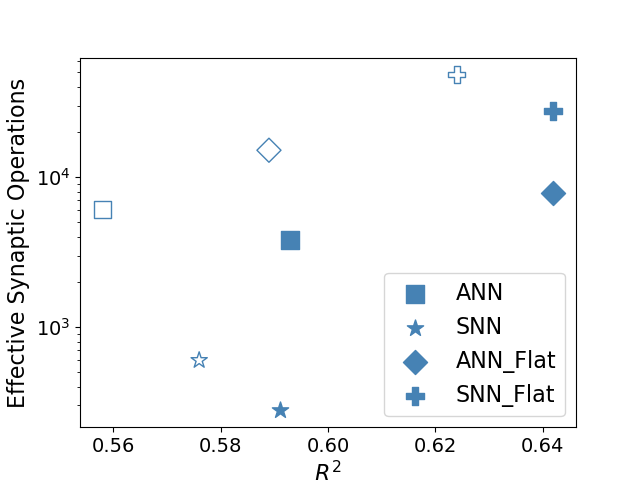
\includegraphics[width=1\linewidth]{figures/Computes_vs_Accuracy.png}
%\caption{A subfigure}
  \label{fig:sub2}
\end{subfigure}
\caption{Footprint and effective synaptic operations vs $R^2$, for four task baselines. Each model has two points: the solid marker represents NHP Indy, and the hollow marker represents NHP Loco.}
\label{fig:motor_result}
\end{figure}

We conduct further exploration for increasing task accuracies with more complex ANN and SNN models: ANN\_Flat and SNN\_Flat. For these networks, 50 data samples of buffered input are split into $n_p=7$ accumulated bins. For ANN\_Flat, the 7 bins are spatially flattened as input to the network, so its topology is ($7\times N_{ch}$)-32-48-2. 
SNN\_Flat uses the $N_{ch}$-32-48-2 topology, and the 7 bins are temporally flattened as input, presented to the network as separate input timesteps. Each prediction still uses the membrane potential of the output neurons after input timesteps, and the network is reset for each prediction. Layer normalization is also applied on the SNN\_Flat inputs.

Figure \ref{fig:motor_result} shows plots of complexity and predictive quality of all four baseline networks. Both flattened networks demonstrate significantly greater $R^2$ performance than the other two networks. However, the larger input dimension of the ANN\_Flat network is reflected in its greater footprint, and the increased model timesteps and layer normalization sharply increase the effective operations of SNN\_Flat by two orders of magnitude compared to the simpler SNN. Thus, while input flattening and normalization increase the quality of model predictions for ANNs and SNNs, each comes with a significant complexity trade-off. 
% Further research is motivated in computationally efficient model performance enhancement, such as weight plasticity or neuron models, that may be directly supported by neuromorphic hardware.



\subsubsection*{Chaotic Function Prediction}
% TODO: need to figure out how to cite and position in terms of existing benchmarking with MG: https://www.sciencedirect.com/science/article/pii/S2666827022000275
% \cite{shahi2022prediction}
% \begin{table}[ht]
% \centerline{
% \renewcommand{\arraystretch}{1.2}
% \begin{tabular}{|c|c|c|c|c|c|ccc|}
% \hline
% \multirow{2}{*}{Baseline} &
%   \multirow{2}{*}{sMAPE} &
%   \multirow{2}{*}{\begin{tabular}[c]{@{}c@{}}Footprint\\ (bytes)\end{tabular}} &
%   \multirow{2}{*}{\begin{tabular}[c]{@{}c@{}}Frequency\\ (Hz)\end{tabular}} &
%   \multirow{2}{*}{\begin{tabular}[c]{@{}c@{}}Connection\\ Sparsity\end{tabular}} &
%   \multirow{2}{*}{\begin{tabular}[c]{@{}c@{}}Activation\\ Sparsity\end{tabular}} &
%   \multicolumn{3}{c|}{SynOps} \\ \cline{7-9} 
%         &       &          &    &     &       & \multicolumn{1}{c|}{Dense}    & \multicolumn{1}{c|}{Eff\_MACs} & Eff\_ACs \\ \hline
% ESN & 14.79 & $2.81 \times 10^5$ & - & 0.876 & 0.0 & \multicolumn{1}{c|}{$3.52 \times 10^{4}$} & \multicolumn{1}{c|}{$4.37 \times 10^{3}$}  & 0 \\ \hline
% LSTM  & 13.37 & $4.90 \times 10^5$ & - & 0.0 & 0.530 & \multicolumn{1}{c|}{$6.03 \times 10^{4}$} & \multicolumn{1}{c|}{$6.03\times 10^{4}$}  & 0 \\ \hline
% \end{tabular}
% }
% \caption{Baseline results for the chaotic function prediction task. Frequency is not reported as the data is a synthetic time-series, with no real time correlation.}
%     \label{tab:MackeyGlass_resuls}
% \end{table}

\begin{table}[ht]
\centerline{
\renewcommand{\arraystretch}{1.3}
\begin{tabular}{c|cccccccc} \thickhline
\multirow{2}{*}{Baseline} &
  \multirow{2}{*}{\begin{tabular}[c]{@{}c@{}}sMAPE\end{tabular}} &
  \multirow{2}{*}{\begin{tabular}[c]{@{}c@{}}Footprint\\ (bytes)\end{tabular}} &
  \multirow{2}{*}{\begin{tabular}[c]{@{}c@{}}Model Exec.\\ Rate (Hz)\end{tabular}} &
  \multirow{2}{*}{\begin{tabular}[c]{@{}c@{}}Connection\\ Sparsity\end{tabular}} &
  \multirow{2}{*}{\begin{tabular}[c]{@{}c@{}}Activation\\ Sparsity\end{tabular}} &
  \multicolumn{3}{c}{SynOps (per model exec.)} \\ \cline{7-9} 
        &       &          &    &     &       & \multicolumn{1}{c}{Dense}    & \multicolumn{1}{c}{Eff\_MACs} & Eff\_ACs \\ \hline
ESN & 14.79 & $2.81 \times 10^5$ & - & 0.876 & 0.0 & \multicolumn{1}{c}{$3.52 \times 10^{4}$} & \multicolumn{1}{c}{$4.37 \times 10^{3}$}  & 0 \\ 
LSTM  & 13.37 & $4.90 \times 10^5$ & - & 0.0 & 0.530 & \multicolumn{1}{c}{$6.03 \times 10^{4}$} & \multicolumn{1}{c}{$6.03\times 10^{4}$}  & 0 \\ \thickhline
\end{tabular}
}
\caption{Baseline results for the chaotic function prediction task. Execution rate is not reported as the data is a synthetic time series, with no real-time correlation.}
    \label{tab:MackeyGlass_resuls}
\end{table}

The chaotic function prediction task has two recurrent ANN baselines, which feature distinct network architectures:

\begin{itemize}
        \item \textbf{Long short-term memory (LSTM)} -- LSTMs are a class of recurrent ANN architectures~\cite{Hochreiter1997}, utilizing multiple gates for selective retention or omission of past information. The LSTM baseline consists of a single LSTM with a hidden state of 100 neurons, followed by a feed-forward layer to produce single-dimension output predictions. 
        In addition, the LSTM baseline utilizes explicit memory by buffering 50 previous datapoints, spatially flattening them into 50 input channels.
        
        \item \textbf{Echo state network (ESN)} -- ESNs are randomized recurrent ANNs that belong to a class of algorithms known collectively as reservoir computing~\cite{ScardapaneRandomness2017}, featuring more biologically-inspired principles than LSTMs despite not being spiking networks. Standard ESNs have only one hidden layer (the reservoir), where synaptic connections projecting input data to the hidden layer and recurrent synaptic connections within the hidden layer are chosen randomly and stay fixed during the training. 
        % The only part of the network that is trained (referred to as the readout matrix) are the connections from the hidden and input layers to the output layer. 
        The model architecture for the ESN baseline has two neurons in the input layer, which projects the Mackey-Glass function input and additional constant bias input into a hidden layer of 186 neurons. Within the hidden layer, the probability of recurrent connections is set to 0.11. 
        % The training of the readout matrix was done using the standard teacher forcing procedure that, for the given time series, collected a matrix with activations of the input and hidden layers of the ESN and a vector with the corresponding ground truth values for the output layer.  This information was used to obtain the readout matrix with the regularized least squares estimator, Methods~\ref{sec:methods:algorithm:baselines}.
        
        
    
    \end{itemize}
The LSTM and ESN models were evaluated on a Mackey-Glass time series with $\tau=17$. The model is evaluated over 30 instantiations of the system; in each instance the start point is shifted forward by half of the Lyapunov time. The model is re-initialized and re-trained on each instance, and the results are averaged over all 30 instances. 

% JY: moved into methods
% The LSTM baseline shares characteristics with other baselines of a high effective-to-dense synaptic operation ratio, with a significant activation sparsity. Here, the internal sigmoid and $\tanh$ functions of the LSTM gates are not considered to be neuron activations, thus activations only account for the ReLU between the final LSTM cell and output layer. 

The ESN model is architecturally unique compared to the other ANN and SNN baselines. The connection sparsity metric ($0.876$) reflects the high number of zero-weight connections across its reservoir hidden layer. Due to this sparsity, hardware with support for sparse synaptic representation by ignoring zero weights would require less memory to represent the network, thus decreasing the deployed footprint of the model. The high connection sparsity of the ESN leads to significant reduction in synaptic operations - the ESN uses an order of magnitude fewer effective operations ($4.37\times10^3)$ than the LSTM ($6.03\times10^4$), while achieving comparable sMAPE. The activation sparsity of the ESN is 0 due to neurons using $\tanh(\cdot)$, rather than ReLU activations.



\begin{figure}[ht]
            \centering
            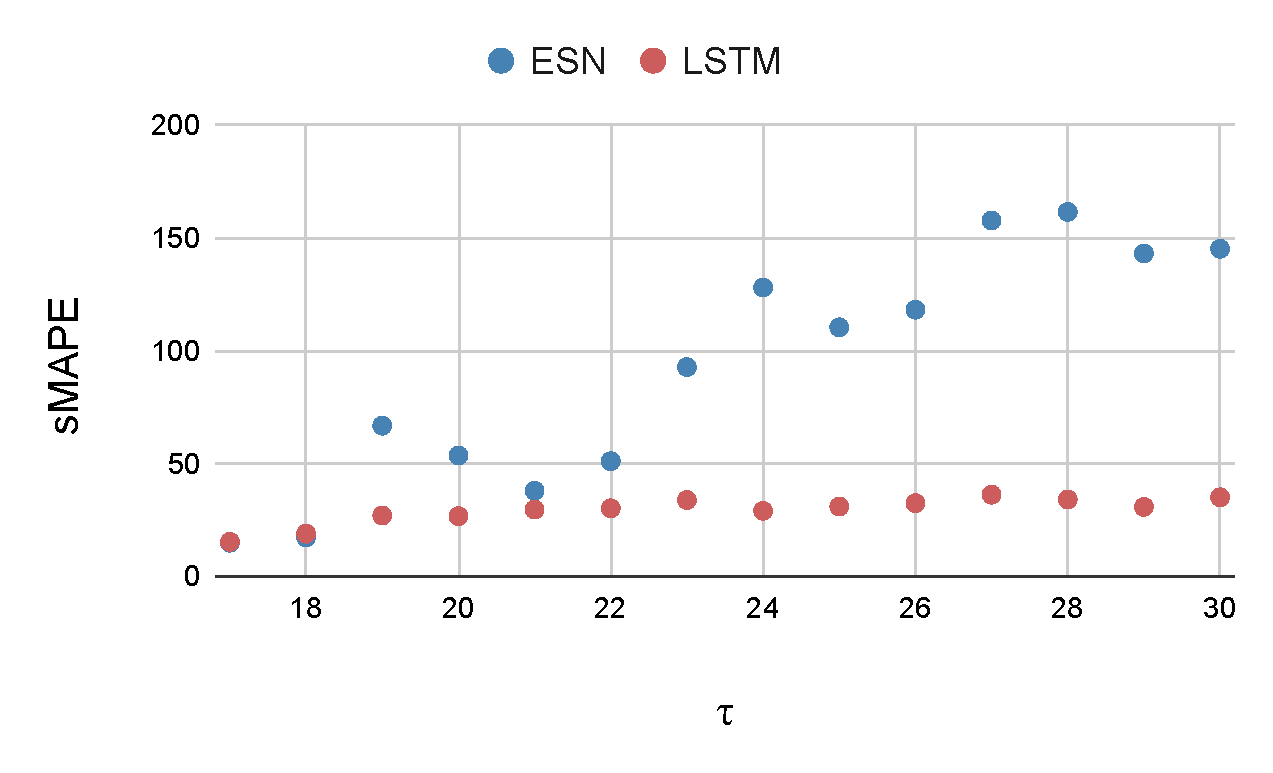
\includegraphics[width=.70\textwidth]{figures/mg_vary_tau.pdf}
            \caption{ESN and LSTM models evaluated on varying Mackey-Glass time series using a constant set of hyperparameters.}
        \label{fig:mackey_glass_function_performance}
    \end{figure}

Furthermore, we show the generalization and robustness capabilities of the particular ESN and LSTM models by applying them, with fixed hyperparameter sets, to other Mackey-Glass time series. Figure \ref{fig:mackey_glass_function_performance} shows the sMAPE score of the models over varied time series with the $\tau$ Mackey-Glass parameter varying between 17 and 30. The models were trained independently for each time series.
As the Mackey-Glass $\tau$ parameter characterizes the time-delay of the system, its increase roughly corresponds to prediction difficulty, shown by the increasing sMAPE trend through the plot. Notably, the LSTM maintains an error that is relatively lower than that of the ESN for all $\tau > 18$. However, the LSTM uses explicit memory via input buffering, so it is conjectured that the historical data allows for greater robustness to the varying time series characteristics. The ESN uses only one previous timestep, so its memory is only implicitly retained within its hidden layer. While the ESN tunes well to the $\tau$=17 case and demonstrates greatly reduced effective operations compared to the LSTM, the same set of hyperparameters does not generalize as well to other time series. Further research is motivated in explicit memory buffers versus implicit memory within the network state for trade-offs in single-series forecasting performance, complexity, and generalization capability.

\subsubsection*{Discussion and Opportunities for Further Research}
Baseline results for the four v1.0 algorithm track tasks compare the correctness and complexities of various solution types. Compared to ANNs, SNNs and ESNs demonstrate complexity advantages such as smaller footprints, high sparsity, and accumulate rather than multiply-and-accumulate operations. Especially on the motor prediction and chaotic function prediction regression tasks, the SNN and ESN baselines already achieve competitive correctness at lower complexity than the ANN and LSTM counterparts. Further research opportunities in model architectures, data pre-processing and buffering, and training paradigms to achieve greater performance is enabled by the standard framework and tooling provided by NeuroBench.